%%%%%%%%%%%%%%%%%%%%%%%%%%%%%%%%%%%%%%%%%%%%%%%%%%%%%%%%%%%%%%%%%%%%%%%%%%%%
% AGUJournalTemplate.tex: this template file is for articles formatted with LaTeX
%
% This file includes commands and instructions
% given in the order necessary to produce a final output that will
% satisfy AGU requirements, including customized APA reference formatting.
%
% You may copy this file and give it your
% article name, and enter your text.
%
% guidelines and troubleshooting are here: 

%% To submit your paper:
\documentclass[draft]{agujournal2019}
\usepackage{url} %this package should fix any errors with URLs in refs.
\usepackage{lineno}
\usepackage[inline]{trackchanges} %for better track changes. finalnew option will compile document with changes incorporated.
\usepackage{soul}
\linenumbers
%%%%%%%
% As of 2018 we recommend use of the TrackChanges package to mark revisions.
% The trackchanges package adds five new LaTeX commands:
%
%  \note[editor]{The note}
%  \annote[editor]{Text to annotate}{The note}
%  \add[editor]{Text to add}
%  \remove[editor]{Text to remove}
%  \change[editor]{Text to remove}{Text to add}
%
% complete documentation is here: http://trackchanges.sourceforge.net/
%%%%%%%

\draftfalse



\journalname{Geophysical Research Letters}


\begin{document}


\title{=enter title here=}


\authors{D. Kennedy\affil{1,2}, D. M. Lawrence\affil{1}, and I. R. Simpson\affil{1}}

\affiliation{1}{Climate and Global Dynamics Laboratory, NSF National Center for Atmospheric Research, Boulder, CO}
\affiliation{2}{Earth Research Institute, University of California Santa Barbara, Santa Barbara, CA}

\correspondingauthor{Daniel Kennedy}{djk2120@ucar.edu}



%  Each must be 140 characters or fewer with no special characters or punctuation and must be complete sentences



\begin{keypoints}
\item enter point 1 here
\item enter point 2 here
\item enter point 3 here
\end{keypoints}



\begin{abstract}
The 2020 Southwest U.S. drought was the driest summer of the instrumented record and part of a 20-year megadrought with severe consequences for water resources. Despite biases in the fully coupled CESM2, we were able to reproduce observed precipitation in a constrained circulation framework, by nudging the large scale circulation to reanalysis winds. Previous work has attributed the precipitation anomalies primarily to natural variability as opposed to radiative forcing or warming. We ported the 2020 circulation pattern to past and future climates to understand if warming influences monsoon period precipitation. Ensemble mean precipitation was 4mm higher under pre-industrial conditions, which is relatively small compared to the 2020 drought anomaly of -66mm, confirming that warming was at most a small contributor to monsoon failure. Ensemble mean precipitation was another 9mm lower under end-of-century conditions, indicating that future warming could further exacerbate Southwest U.S. droughts. However, we found that our future conditions constrained circulation ensemble was significantly drier than any simulations in a fully coupled framework, indicating that large-scale feedbacks may disallow this circulation pattern in the future.
\end{abstract}

\section*{Plain Language Summary}
Enter your Plain Language Summary here or delete this section.
Here are instructions on writing a Plain Language Summary: 
https://www.agu.org/Share-and-Advocate/Share/Community/Plain-language-summary


%%%%%%%%%%%%%%%%%%%%%%%%%%%%%%%%%%%%%%%%%%%%%%%
%
%  BODY TEXT
%
%%%%%%%%%%%%%%%%%%%%%%%%%%%%%%%%%%%%%%%%%%%%%%%


\section{Introduction}



Coupled ESMs have not captured humidity trends in semi-arid ecosystems \cite{simpson2024}.

Though ESMs show a slight increase in spring precipitation in the region, there does not seem to be an attributable influence of climate change on NAM precipitation. Previous work indicates that the 2020 SWUS drought was not exacerbated by climate change, but was rather a result of  internal atmospheric variability \cite{seager2022}. 

\section{Methods}

\section{Results and Discussion}
\subsection{Simulating the 2020 SWUS drought}

\subsection{Porting the 2020 circulation to past and future climates}

\subsection{Similarities and differences between the CCE and the CESM2-LE}
ET$\sim$SM looks the same. But P$\sim$ET looks a bit different. The CCE mean looks to be in a reasonable spot, roughly speaking, but the partial response of P to varying ET (via land initialization) looks much smaller than in the fully coupled model. This would seem to indicate that the coupling of SM->ET is agnostic to the broader circulation, whereas P is not simply determined by the local ET. In the coupled model we tend to see an 18mm reduction in P for a 10mm reduction in ET, but in the CCE it looks more like 5mm P per 10mm ET. In the coupled model the circulation associated with 140mm ET may be quite different from the circulation that results in 120mm ET, in addition to any differences in the initial conditions. In the CCE, only the initial conditions are different, and the large-scale circulation is following observations. When CCE goes from ET of 120 to 100, the broader circulation still provides a relatively equivalent flux of water to the region (in fact slightly higher), which helps support the precipitation from falling drastically. In the coupled model, when ET goes from 140 to 120mm, it is probably largely driven by a change to a more diverging circulation, whereby the precip is robbed of the convergence flux as well as the associated reductions in ET flux. 

Does this invalidate inference from the CCE? No, it just means that any takeaways are conditional to the given circulation pattern. In the case of understanding sensitivity to initial conditions in the 2020 ensemble, the experimental framework is probably quite helpful. In the case of the analogue simulations, it's slightly more complicated, because warmer or colder climates may not be able to develop this circulation pattern. Towards this end, the fact that the 2090 ensemble is so much drier than anything seen in the fully coupled model is hard to overlook. This would seem to indicate that CESM2 predicts changes in circulation that would disallow the droughts we are simulating in the 2090 CCE. Further work to understand the mechanisms underpinning may be interesting, especially given the tendency across many coupled models to produce aberrant VP trends in semi-arid ecosystems. 


Why is the CCE drier than the LE in 2090?


\subsection{Inference capabilities for extreme droughts}


\begin{figure}
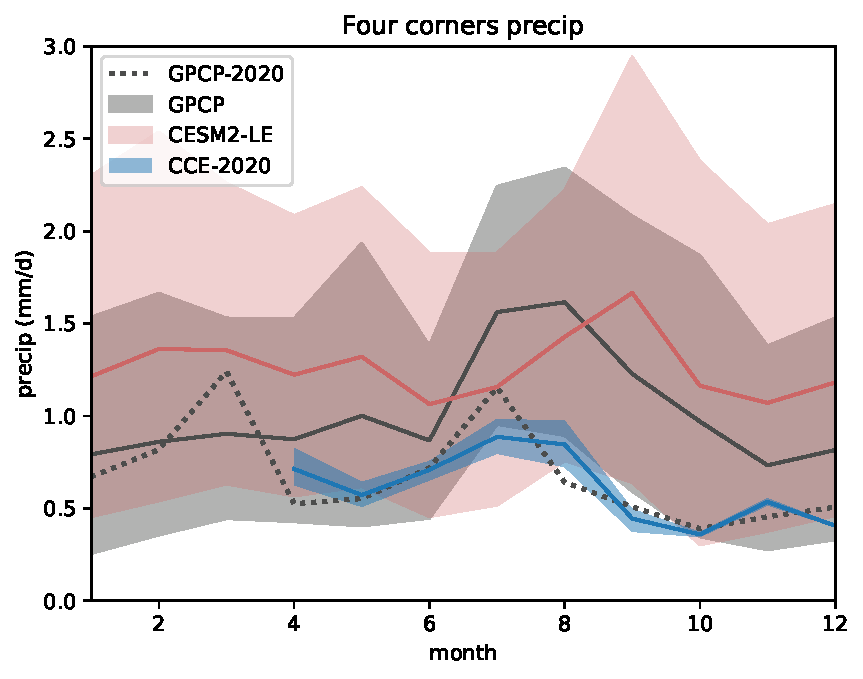
\includegraphics[width=30pc]{../figs/main/precip.pdf}
\caption{The constrained circulation ensemble provides a reasonable match for precipitation observations during the 2020 SWUS drought, despite  biases in the fully coupled model. Shaded areas span the 5th to 95th percentiles across pooled ensemble-years (CESM2: 1980-2020, CCE: 2020 only), or in the case of the GPCP observational product, simply across years (1980-2020). Solid lines denote the climatological averages. The GPCP observed precipitation during 2020 is shown as the dotted line. Additional panel with experimental protocol and perhaps some dynamical notion tk.}
\end{figure}

\begin{figure}
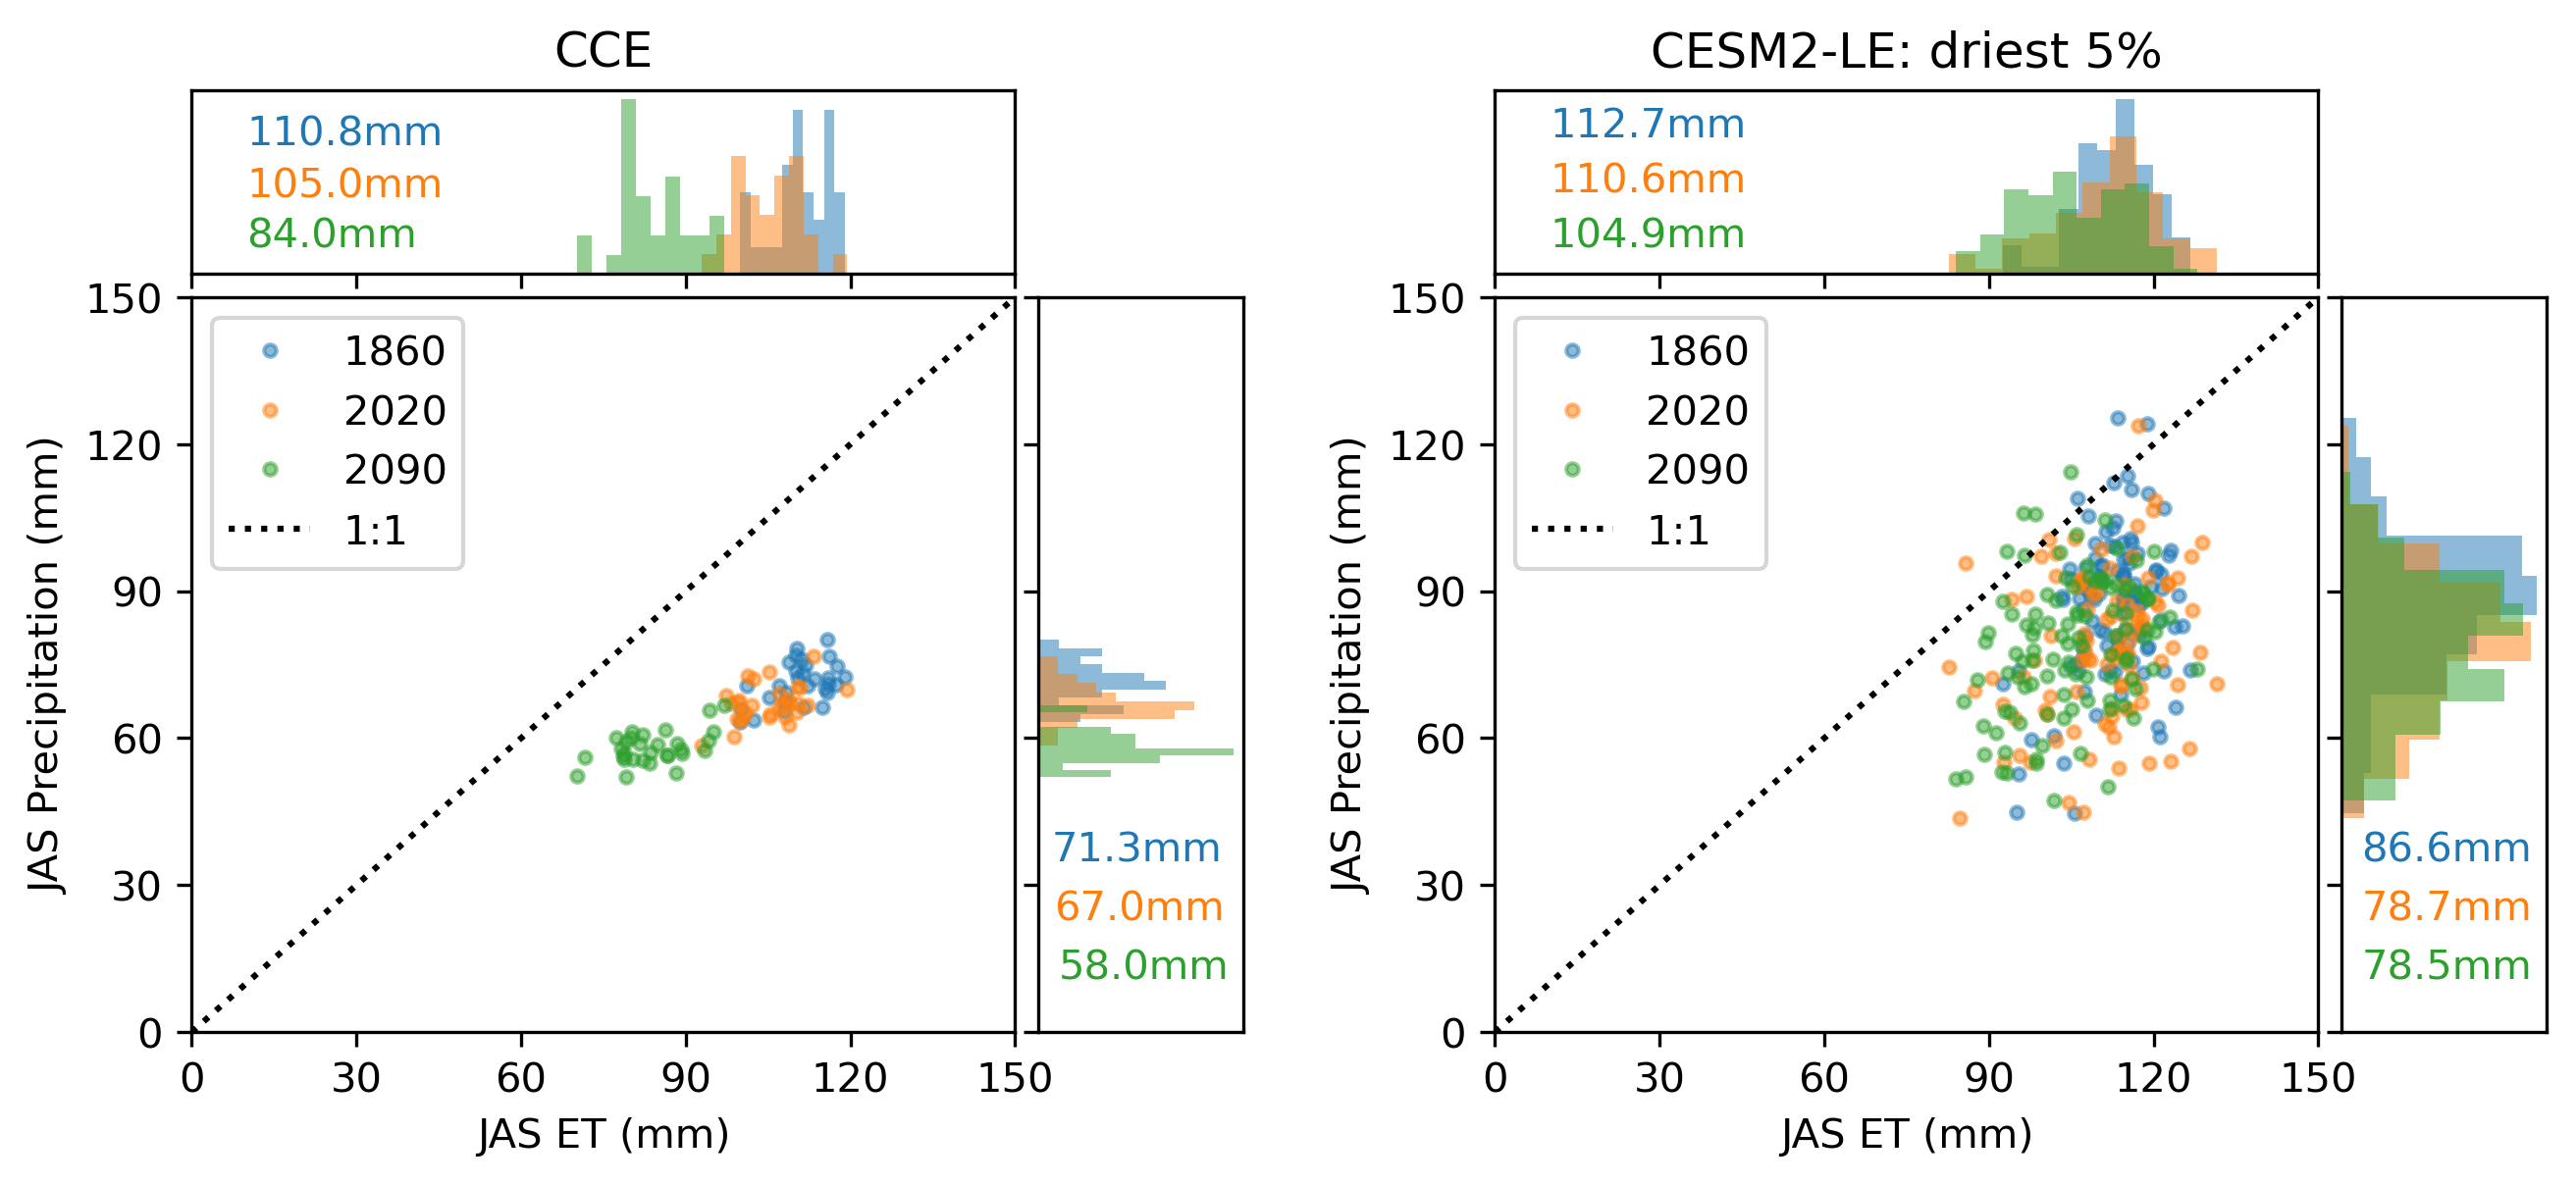
\includegraphics[width=40pc]{../figs/main/scatter_ET_P.png}
\caption{Monsoon period precipitation vs. ET in the CCE and a dry subset of the CESM2-LE from three different time periods. ET and Precip seem to decline in both ensembles in response to climate change forcing. Printed numbers indicate the various ensemble means. Two asterisks indicate a given ensemble mean is distinguishable from both the other time period means at the p$<$0.05 level. One asterisk indicates it is distinguishable from just one of the other time periods. The dry subset of the CESM2-LE is defined as the 3\% driest ensemble years from the given time period based on JAS 10cm soil moisture (see methods). Relabeled as 1850 tk.}
\end{figure}

\begin{figure}
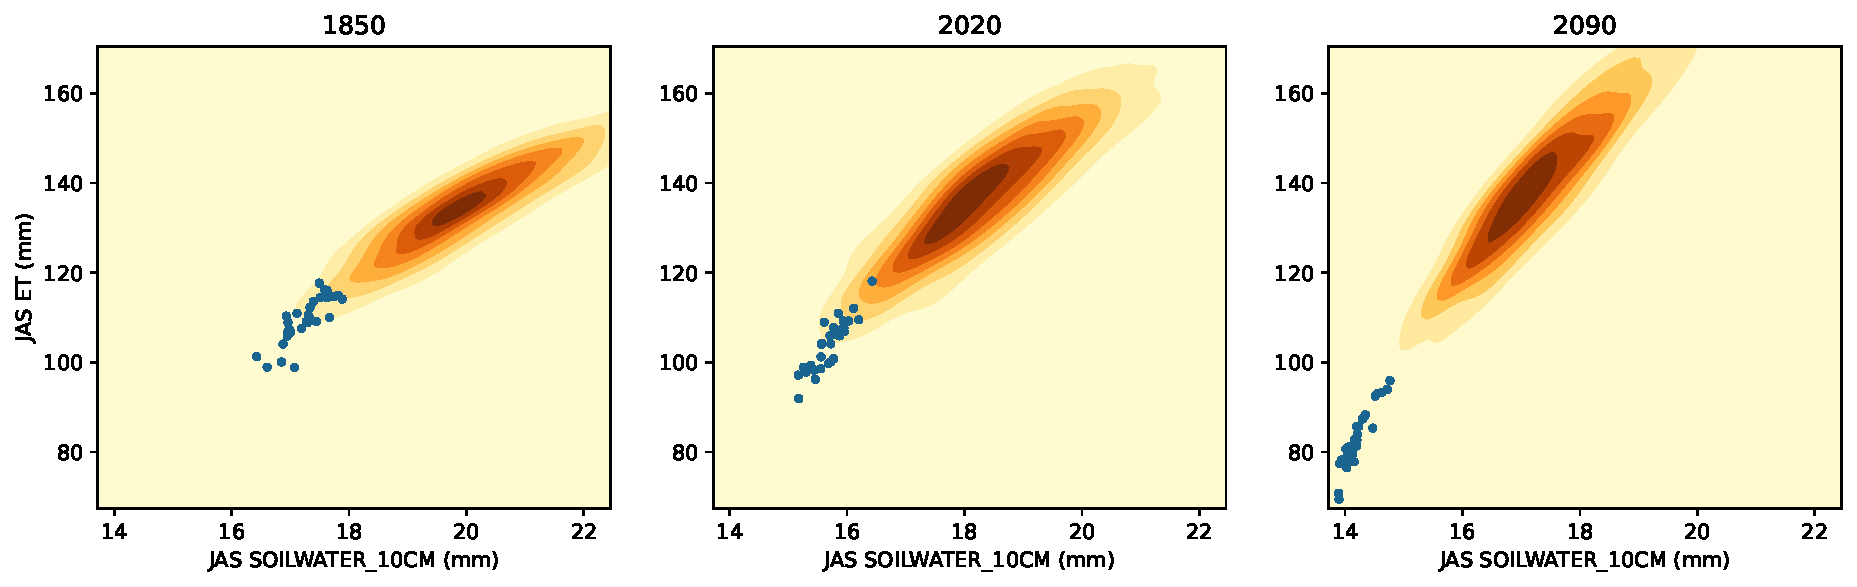
\includegraphics[width=35pc]{../figs/main/contours_ET_SW.pdf}
\caption{Soil moisture (10cm) vs. ET in the CCE (dots) and the CESM2-LE (scatter density heat map) for three time periods. The CCE appears fully consistent with the coupled model with regard to this relationship, demonstrating an intensification of the hydrological cycle in the region. Note that the CCE does however appear significantly drier relative to the LE in 2090 as compared to 1850 or 2020. A second set of plots with something less clean looking potentially tk.}
\end{figure}


\begin{figure}
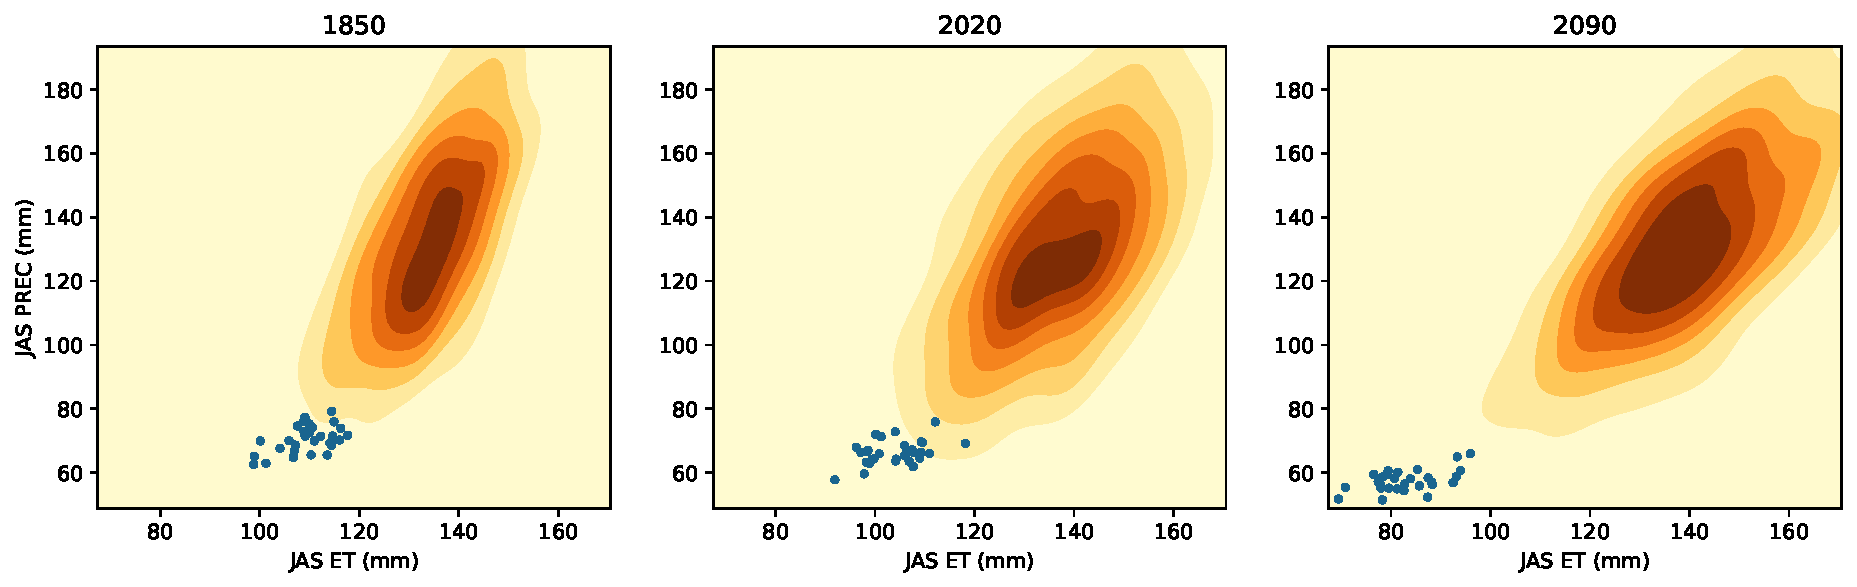
\includegraphics[width=35pc]{../figs/main/contours_PREC_ET.pdf}
\caption{Soil moisture (10cm) vs. ET in the CCE (dots) and the CESM2-LE (scatter density heat map) for three time periods. The CCE appears fully consistent with the coupled model with regard to this relationship, demonstrating an intensification of the hydrological cycle in the region. Note that the CCE does however appear significantly drier relative to the LE in 2090 as compared to 1850 or 2020. A second set of plots with something less clean looking potentially tk.}
\end{figure}


\begin{figure}
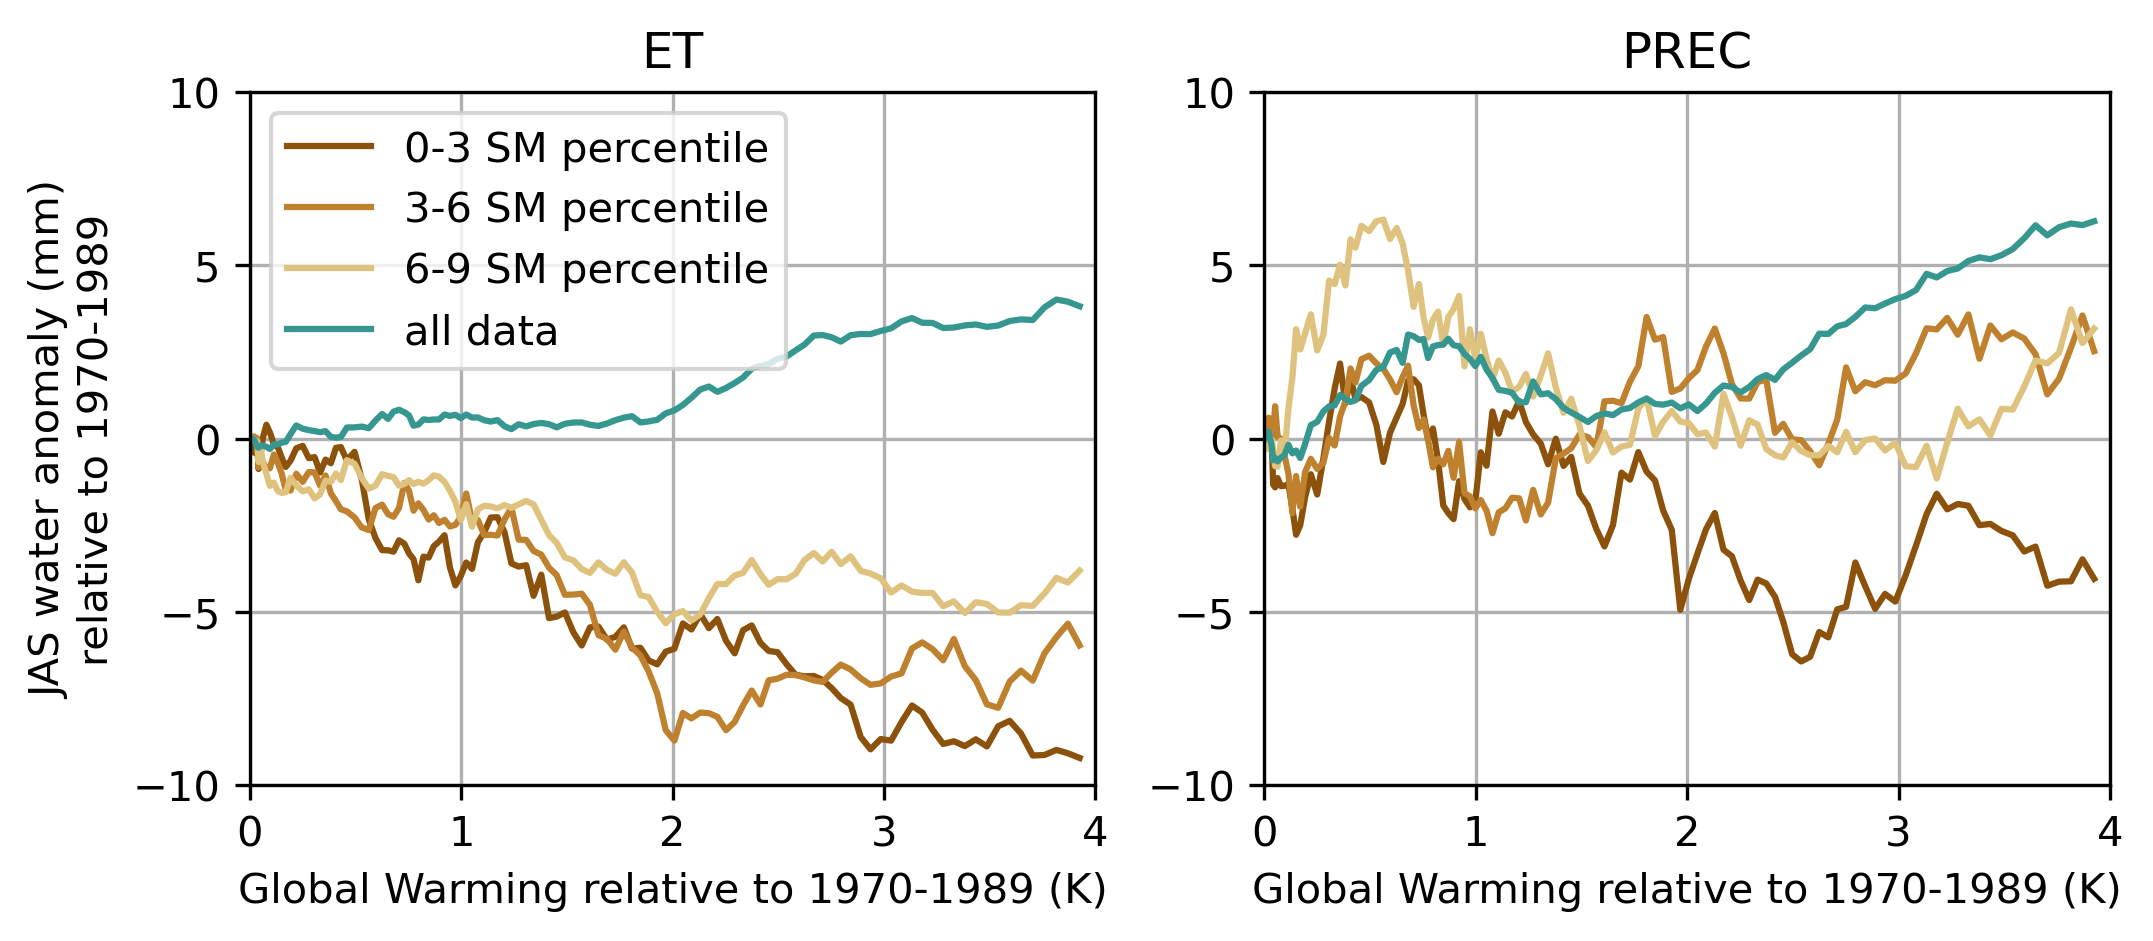
\includegraphics[width=40pc]{../figs/main/cesm2le_water_anomalies.png}
\caption{Monsoon period precipitation and ET anomalies (relative to 1970-1989) from the CESM2-LE from various ensemble subsets delineated based on 10cm soil moisture. Whereas the ensemble mean (turquoise) shows increases in precipitation and ET, the drier subsets can feature decreases. For reference, CESM2 climatological precipitation and ET are XX and YYmm. Refigured with non-overlapping composites tk.}
\end{figure}



\section{Conclusions}

%%

%  Numbered lines in equations:
%  To add line numbers to lines in equations,
%  \begin{linenomath*}
%  \begin{equation}
%  \end{equation}
%  \end{linenomath*}



%% Enter Figures and Tables near as possible to where they are first mentioned:
%
% DO NOT USE \psfrag or \subfigure commands.
%
% Figure captions go below the figure.
% Acronyms used in figure captions will be spelled out in the final, published version.

% Table titles go above tables;  other caption information
%  should be placed in last line of the table, using
% \multicolumn2l{$^a$ This is a table note.}
% NOTE that there is no difference between table caption and table heading in the final, published version
%
%----------------
% EXAMPLE FIGURES
%
% \begin{figure}
% \includegraphics{example.png}
% \caption{caption}
% \end{figure}
%
% Giving latex a width will help it to scale the figure properly. A simple trick is to use \textwidth. Try this if large figures run off the side of the page.
% \begin{figure}
% \noindent\includegraphics[width=\textwidth]{anothersample.png}
%\caption{caption}
%\label{pngfiguresample}
%\end{figure}
%
%
% If you get an error about an unknown bounding box, try specifying the width and height of the figure with the natwidth and natheight options. This is common when trying to add a PDF figure without pdflatex.
% \begin{figure}
% \noindent\includegraphics[natwidth=800px,natheight=600px]{samplefigure.pdf}
%\caption{caption}
%\label{pdffiguresample}
%\end{figure}
%
%
% PDFLatex does not seem to be able to process EPS figures. You may want to try the epstopdf package.
%

%
% ---------------
% EXAMPLE TABLE
%
% \begin{table}
% \caption{Time of the Transition Between Phase 1 and Phase 2$^{a}$}
% \centering
% \begin{tabular}{l c}
% \hline
%  Run  & Time (min)  \\
% \hline
%   $l1$  & 260   \\
%   $l2$  & 300   \\
%   $l3$  & 340   \\
%   $h1$  & 270   \\
%   $h2$  & 250   \\
%   $h3$  & 380   \\
%   $r1$  & 370   \\
%   $r2$  & 390   \\
% \hline
% \multicolumn{2}{l}{$^{a}$Footnote text here.}
% \end{tabular}
% \end{table}

%%%%%%%%%%%%%%%%%%%%%%%%%%%%%%%%%%%%%%%%%%%%%%%
% SIDEWAYS FIGURES and TABLES
% AGU prefers the use of {sidewaystable} over {landscapetable} as it causes fewer problems.
%
% \begin{sidewaysfigure}
% \includegraphics[width=20pc]{figsamp}
% \caption{caption here}
% \label{newfig}
% \end{sidewaysfigure}
%
%  \begin{sidewaystable}
%  \caption{Caption here}
% \label{tab:signif_gap_clos}
%  \begin{tabular}{ccc}
% one&two&three\\
% four&five&six
%  \end{tabular}
%  \end{sidewaystable}

%% If using numbered lines, please surround equations with \begin{linenomath*}...\end{linenomath*}
%\begin{linenomath*}
%\begin{equation}
%y|{f} \sim g(m, \sigma),
%\end{equation}
%\end{linenomath*}

%%% End of body of article

%%%%%%%%%%%%%%%%%%%%%%%%%%%%%%%%%%%%%%%%%%%%%%%
%% Optional Appendices go here
%
% The \appendix command resets counters and redefines section heads
%
% After typing \appendix
%
%\section{Here Is Appendix Title}
% will show
% A: Here Is Appendix Title
%
%\appendix
%\section{Here is a sample appendix}

%%%%%%%%%%%%%%%%%%%%%%%%%%%%%%%%%%%%%%%%%%%%%%%
% Optional Glossary, Notation or Acronym section goes here:
%
% Glossary is only allowed in Reviews of Geophysics
%  \begin{glossary}
%  \term{Term}
%   Term Definition here
%  \term{Term}
%   Term Definition here
%  \term{Term}
%   Term Definition here
%  \end{glossary}


%%%%%%%%%%%%%%%%%%%%%%%%%%%%%%%%%%%%%%%%%%%%%%%
% Acronyms
%% NOTE that acronyms in the final published version will be spelled out when used in figure captions.
%   \begin{acronyms}
%   \acro{Acronym}
%   Definition here
%   \acro{EMOS}
%   Ensemble model output statistics
%   \acro{ECMWF}
%   Centre for Medium-Range Weather Forecasts
%   \end{acronyms}


%%%%%%%%%%%%%%%%%%%%%%%%%%%%%%%%%%%%%%%%%%%%%%%
% Notation
%   \begin{notation}
%   \notation{$a+b$} Notation Definition here
%   \notation{$e=mc^2$}
%   Equation in German-born physicist Albert Einstein's theory of special
%  relativity that showed that the increased relativistic mass ($m$) of a
%  body comes from the energy of motion of the body—that is, its kinetic
%  energy ($E$)—divided by the speed of light squared ($c^2$).
%   \end{notation}




%%%%%%%%%%%%%%%%%%%%%%%%%%%%%%%%%%%%%%%%%%%%%%%
%
% DATA SECTION and ACKNOWLEDGMENTS
%
%%%%%%%%%%%%%%%%%%%%%%%%%%%%%%%%%%%%%%%%%%%%%%%

\section*{Open Research Section}
This section MUST contain a statement that describes where the data supporting the conclusions can be obtained. Data cannot be listed as ''Available from authors'' or stored solely in supporting information. Citations to archived data should be included in your reference list. Wiley will publish it as a separate section on the paper’s page. Examples and complete information are here:
https://www.agu.org/Publish with AGU/Publish/Author Resources/Data for Authors


\acknowledgments
Enter acknowledgments here. This section is to acknowledge funding, thank colleagues, enter any secondary affiliations, and so on.




%%%%%%%%%%%%%%%%%%%%%%%%%%%%%%%%%%%%%%%%%%%%%%%
% REFERENCES and BIBLIOGRAPHY
%
% \bibliography{<name of your .bib file>} don't specify the file extension
% don't specify bibliographystyle
%
%%%%%%%%%%%%%%%%%%%%%%%%%%%%%%%%%%%%%%%%%%%%%%%

\bibliography{refs.bib}



%Reference citation instructions and examples:
%
% Please use ONLY \cite and \citeA for reference citations.
% \cite for parenthetical references
% ...as shown in recent studies (Simpson et al., 2019)
% \citeA for in-text citations
% ...Simpson et al. (2019) have shown...
%
%
%...as shown by \citeA{jskilby}.
%...as shown by \citeA{lewin76}, \citeA{carson86}, \citeA{bartoldy02}, and \citeA{rinaldi03}.
%...has been shown \cite{jskilbye}.
%...has been shown \cite{lewin76,carson86,bartoldy02,rinaldi03}.
%... \cite <i.e.>[]{lewin76,carson86,bartoldy02,rinaldi03}.
%...has been shown by \cite <e.g.,>[and others]{lewin76}.
%
% apacite uses < > for prenotes and [ ] for postnotes
% DO NOT use other cite commands (e.g., \citet, \citep, \citeyear, \nocite, \citealp, etc.).
%



\end{document}



More Information and Advice:

%%%%%%%%%%%%%%%%%%%%%%%%%%%%%%%%%%%%%%%%%%%%%%%
%
%  SECTION HEADS
%
%%%%%%%%%%%%%%%%%%%%%%%%%%%%%%%%%%%%%%%%%%%%%%%

% Capitalize the first letter of each word (except for
% prepositions, conjunctions, and articles that are
% three or fewer letters).

% AGU follows standard outline style; therefore, there cannot be a section 1 without
% a section 2, or a section 2.3.1 without a section 2.3.2.
% Please make sure your section numbers are balanced.
% ---------------
% Level 1 head
%
% Use the \section{} command to identify level 1 heads;
% type the appropriate head wording between the curly
% brackets, as shown below.
%
%An example:
%\section{Level 1 Head: Introduction}
%
% ---------------
% Level 2 head
%
% Use the \subsection{} command to identify level 2 heads.
%An example:
%\subsection{Level 2 Head}
%
% ---------------
% Level 3 head
%
% Use the \subsubsection{} command to identify level 3 heads
%An example:
%\subsubsection{Level 3 Head}
%
%---------------
% Level 4 head
%
% Use the \subsubsubsection{} command to identify level 3 heads
% An example:
%\subsubsubsection{Level 4 Head} An example.
%
%%%%%%%%%%%%%%%%%%%%%%%%%%%%%%%%%%%%%%%%%%%%%%%
%
%  IN-TEXT LISTS
%
%%%%%%%%%%%%%%%%%%%%%%%%%%%%%%%%%%%%%%%%%%%%%%%
%
% Do not use bulleted lists; enumerated lists are okay.
% \begin{enumerate}
% \item
% \item
% \item
% \end{enumerate}
%
%%%%%%%%%%%%%%%%%%%%%%%%%%%%%%%%%%%%%%%%%%%%%%%
%
%  EQUATIONS
%
%%%%%%%%%%%%%%%%%%%%%%%%%%%%%%%%%%%%%%%%%%%%%%%

% Single-line equations are centered.
% Equation arrays will appear left-aligned.

Math coded inside display math mode \[ ...\]
 will not be numbered, e.g.,:
 \[ x^2=y^2 + z^2\]

 Math coded inside \begin{equation} and \end{equation} will
 be automatically numbered, e.g.,:
 \begin{equation}
 x^2=y^2 + z^2
 \end{equation}


% To create multiline equations, use the
% \begin{eqnarray} and \end{eqnarray} environment
% as demonstrated below.
\begin{eqnarray}
  x_{1} & = & (x - x_{0}) \cos \Theta \nonumber \\
        && + (y - y_{0}) \sin \Theta  \nonumber \\
  y_{1} & = & -(x - x_{0}) \sin \Theta \nonumber \\
        && + (y - y_{0}) \cos \Theta.
\end{eqnarray}

%If you don't want an equation number, use the star form:
%\begin{eqnarray*}...\end{eqnarray*}

% Break each line at a sign of operation
% (+, -, etc.) if possible, with the sign of operation
% on the new line.

% Indent second and subsequent lines to align with
% the first character following the equal sign on the
% first line.

% Use an \hspace{} command to insert horizontal space
% into your equation if necessary. Place an appropriate
% unit of measure between the curly braces, e.g.
% \hspace{1in}; you may have to experiment to achieve
% the correct amount of space.


%%%%%%%%%%%%%%%%%%%%%%%%%%%%%%%%%%%%%%%%%%%%%%%
%
%  EQUATION NUMBERING: COUNTER
%
%%%%%%%%%%%%%%%%%%%%%%%%%%%%%%%%%%%%%%%%%%%%%%%

% You may change equation numbering by resetting
% the equation counter or by explicitly numbering
% an equation.

% To explicitly number an equation, type \eqnum{}
% (with the desired number between the brackets)
% after the \begin{equation} or \begin{eqnarray}
% command.  The \eqnum{} command will affect only
% the equation it appears with; LaTeX will number
% any equations appearing later in the manuscript
% according to the equation counter.
%

% If you have a multiline equation that needs only
% one equation number, use a \nonumber command in
% front of the double backslashes (\\) as shown in
% the multiline equation above.

% If you are using line numbers, remember to surround
% equations with \begin{linenomath*}...\end{linenomath*}

%  To add line numbers to lines in equations:
%  \begin{linenomath*}
%  \begin{equation}
%  \end{equation}
%  \end{linenomath*}



